\cleartorightpage
\begin{savequote}[75mm]
``This job is a great scientific adventure. But it's also a great human adventure. Mankind has made giant steps forward. However, what we know is really very, very little compared to what we still have to know.''
\qauthor{Fabiola Gianotti}
\end{savequote}


\chapter{Introduction}\label{introduction}
 % start numberings at 0 because (computer) science
\setcounter{figure}{-1}
\setcounter{table}{-1}
\setcounter{section}{-1}
\setcounter{NAT@ctr}{-1}

\setlength\parindent{0pt}

\begin{justify}

\section{The Source Code of Life}

DNA\@. The blueprint of life. These long double-stranded helical molecules are present in all living cells on earth\footnote{Some viruses contain only RNA, but these are often not considered `alive'.} and encode the proteins which drive the functioning, structure and replication of the cells and tissues that make up an organism. In many ways, DNA is also analogous to computer code; any computer program, no matter how complex, can be described as a long series of just two characters, \verb+0+ and \verb+1+, known as \emph{bits}. Knowing the sequence of these bits and, crucially, the details about how they are being interpreted by the machine on which they are executed, enables us to understand and predict the functions they encode. In much the same way, DNA uses just 4 different elements, called \emph{bases} or \emph{nucleotides}, to encode its blueprint for the cell. These 4 building blocks are adenine, cytosine, guanine and thymine, usually referred to simply by their first letters, \verb+A+, \verb+C+, \verb+G+ and \verb+T+. These bases combine together in pairs (\emph{base pairs}), with \verb+A+ always matching to \verb+T+ and \verb+C+ being complementary to \verb+G+ along a sugar phosphate backbone in their double-helix configuration (Figure~\ref{fig:dnastructure}). Using continually improving and increasingly affordable genome sequencing techniques, are now able to read this string of bases that make up the cell's blueprint, but unravelling the mysteries of how these are being interpreted by the cell poses a far greater challenge.

\end{justify}


\begin{wrapfigure}{r}{210pt}
%\begin{figure}[h!]
    \centering
    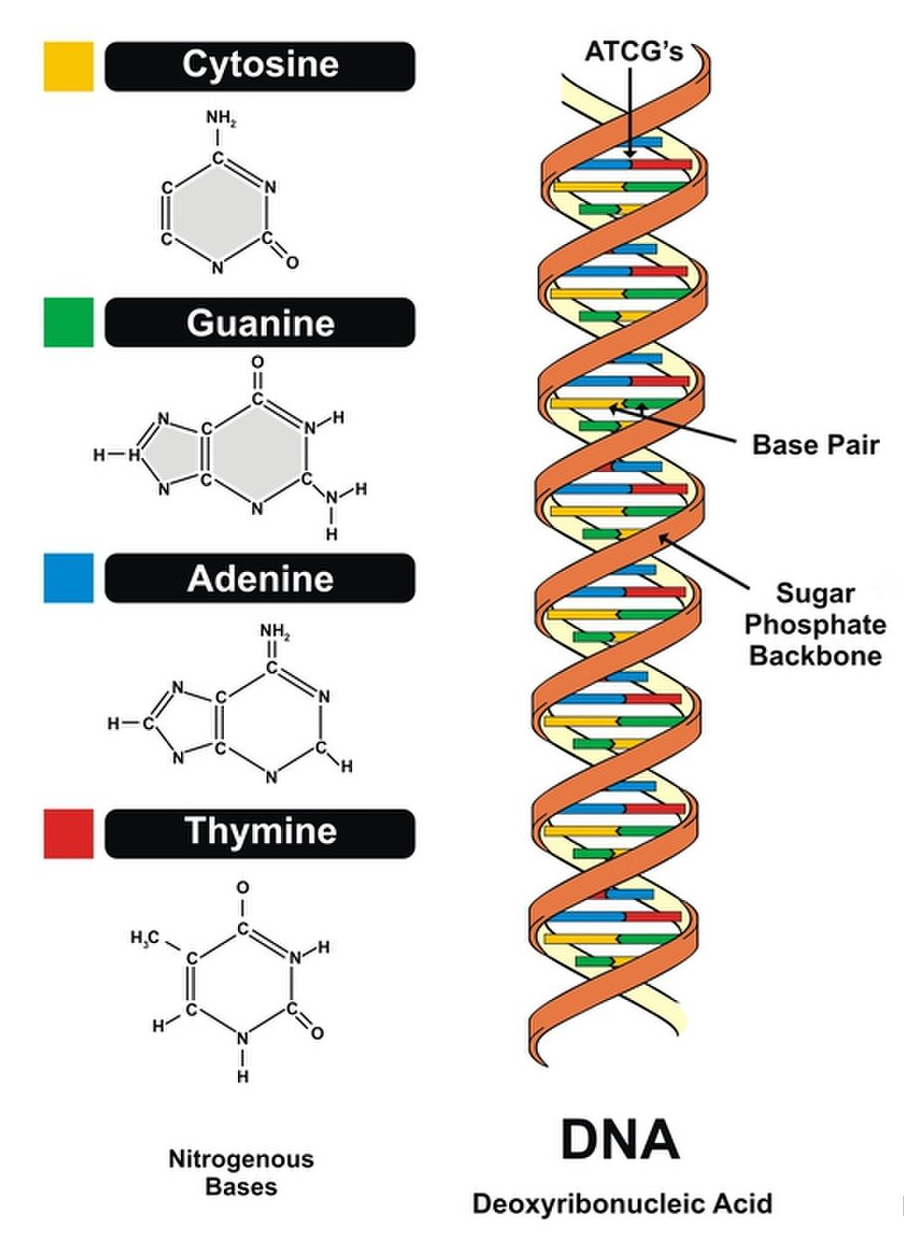
\includegraphics[width=200pt]{chapters/images/introduction/dna-structure.png}
    \caption{Structure of DNA}\label{fig:dnastructure}
%\end{figure}
\end{wrapfigure}

In humans, DNA is organised into 23 pairs of chromosomes, with a total length of approximately 6.4 billion base pairs. Sprinkled across these chromosomes are \emph{genes}; stretches of DNA which often encode protein molecules. When these protein-coding genes are expressed, the gene sequence is transcribed to a messenger molecule (\emph{mRNA}) which is subsequently translated into a protein molecule. About 1\% of the total DNA consists of \emph{exons}, the portions of genes that directly encode protein sequences. The function of the remaining 99\% of the genome long remained a mystery, and was even referred to as \emph{junk DNA}. More recent studies have revealed that many of these stretches of non-coding DNA play an important role in the regulation of the expression of genes, stimulating or prohibiting the translation of genes to proteins and thereby influencing the functioning of the cell. For any two individuals, the vast majority of their DNA sequence will be identical, but small variations in the remaining locations of the genome are what make each of us unique. However, if these variations occur in the wrong place, it also has the potential to cause illness. Studying this natural variation in the genome sequence helps us unravel the mechanisms of life and disease.

\begin{justify}
\subsection{A Brief History of Genome Sequencing}
Friedrich Miescher was the first to isolate DNA molecules (which he termed \emph{nuclein}) in 1869. However, the molecule remained relatively understudied until Rosalind Franklin used X-ray crystallography to inspect the molecule's structure~\cite{elkin2003rosalind}. Watson and Crick famously used this data to postulate the double-helix model of DNA in 1953~\cite{watson1953molecular}. This model illustrated for the first time that DNA molecules were ideally suited for replication, and solidified the idea that DNA, and not protein as was previously thought, was the primary carrier of hereditary information. Simultaneously, Frederick Sanger had developed techniques to sequence proteins, and later RNA and DNA molecules. This was the start of the \emph{first generation} of genome sequencing, and the first full gene was sequenced in 1972, followed by the first full genome in 1976 (bacteriophage ϕX174, 5386 nucleotides long)~\cite{sanger1977dna}. These early techniques were only suitable for relatively small sections of DNA, and more technological advances would be required before larger genomes could be fully sequenced with greater coverage.

In 1990, the Human Genome Project~\cite{olson1993human} set out to sequence the entire 3.2-billion-basepair-long human genome, an effort culminating in 2003 with the publication of the first human \textit{reference genome}~\cite{international2004finishing}. Not only did this provide invaluable insights into human genetics, but it also paved the way for the next era in genetic research; something which would completely transform the field of genetic research. Over the next several years, \emph{next-generation} massively parallel sequencers were developed by companies like Roche454, Solexa, Complete Genomics, Illumina, and others, dramatically cutting the cost and time required to sequence a human genome, and for the first time demonstrated its potential utility in clinical and diagnostic settings. Through sustained technological advancements over the following years, these costs continued to decrease at exponential rates - outstripping even the pace predicted by Moore's law (\hyperref[fig:seqcost]{Figure~\ref{fig:seqcost}}) - and the long dreamed-about \textit{\$1,000 dollar genome}~\cite{thousanddollargenome, sequencingcostsNHGRI} has now become a reality.

\begin{figure}[h!]
    \centering
    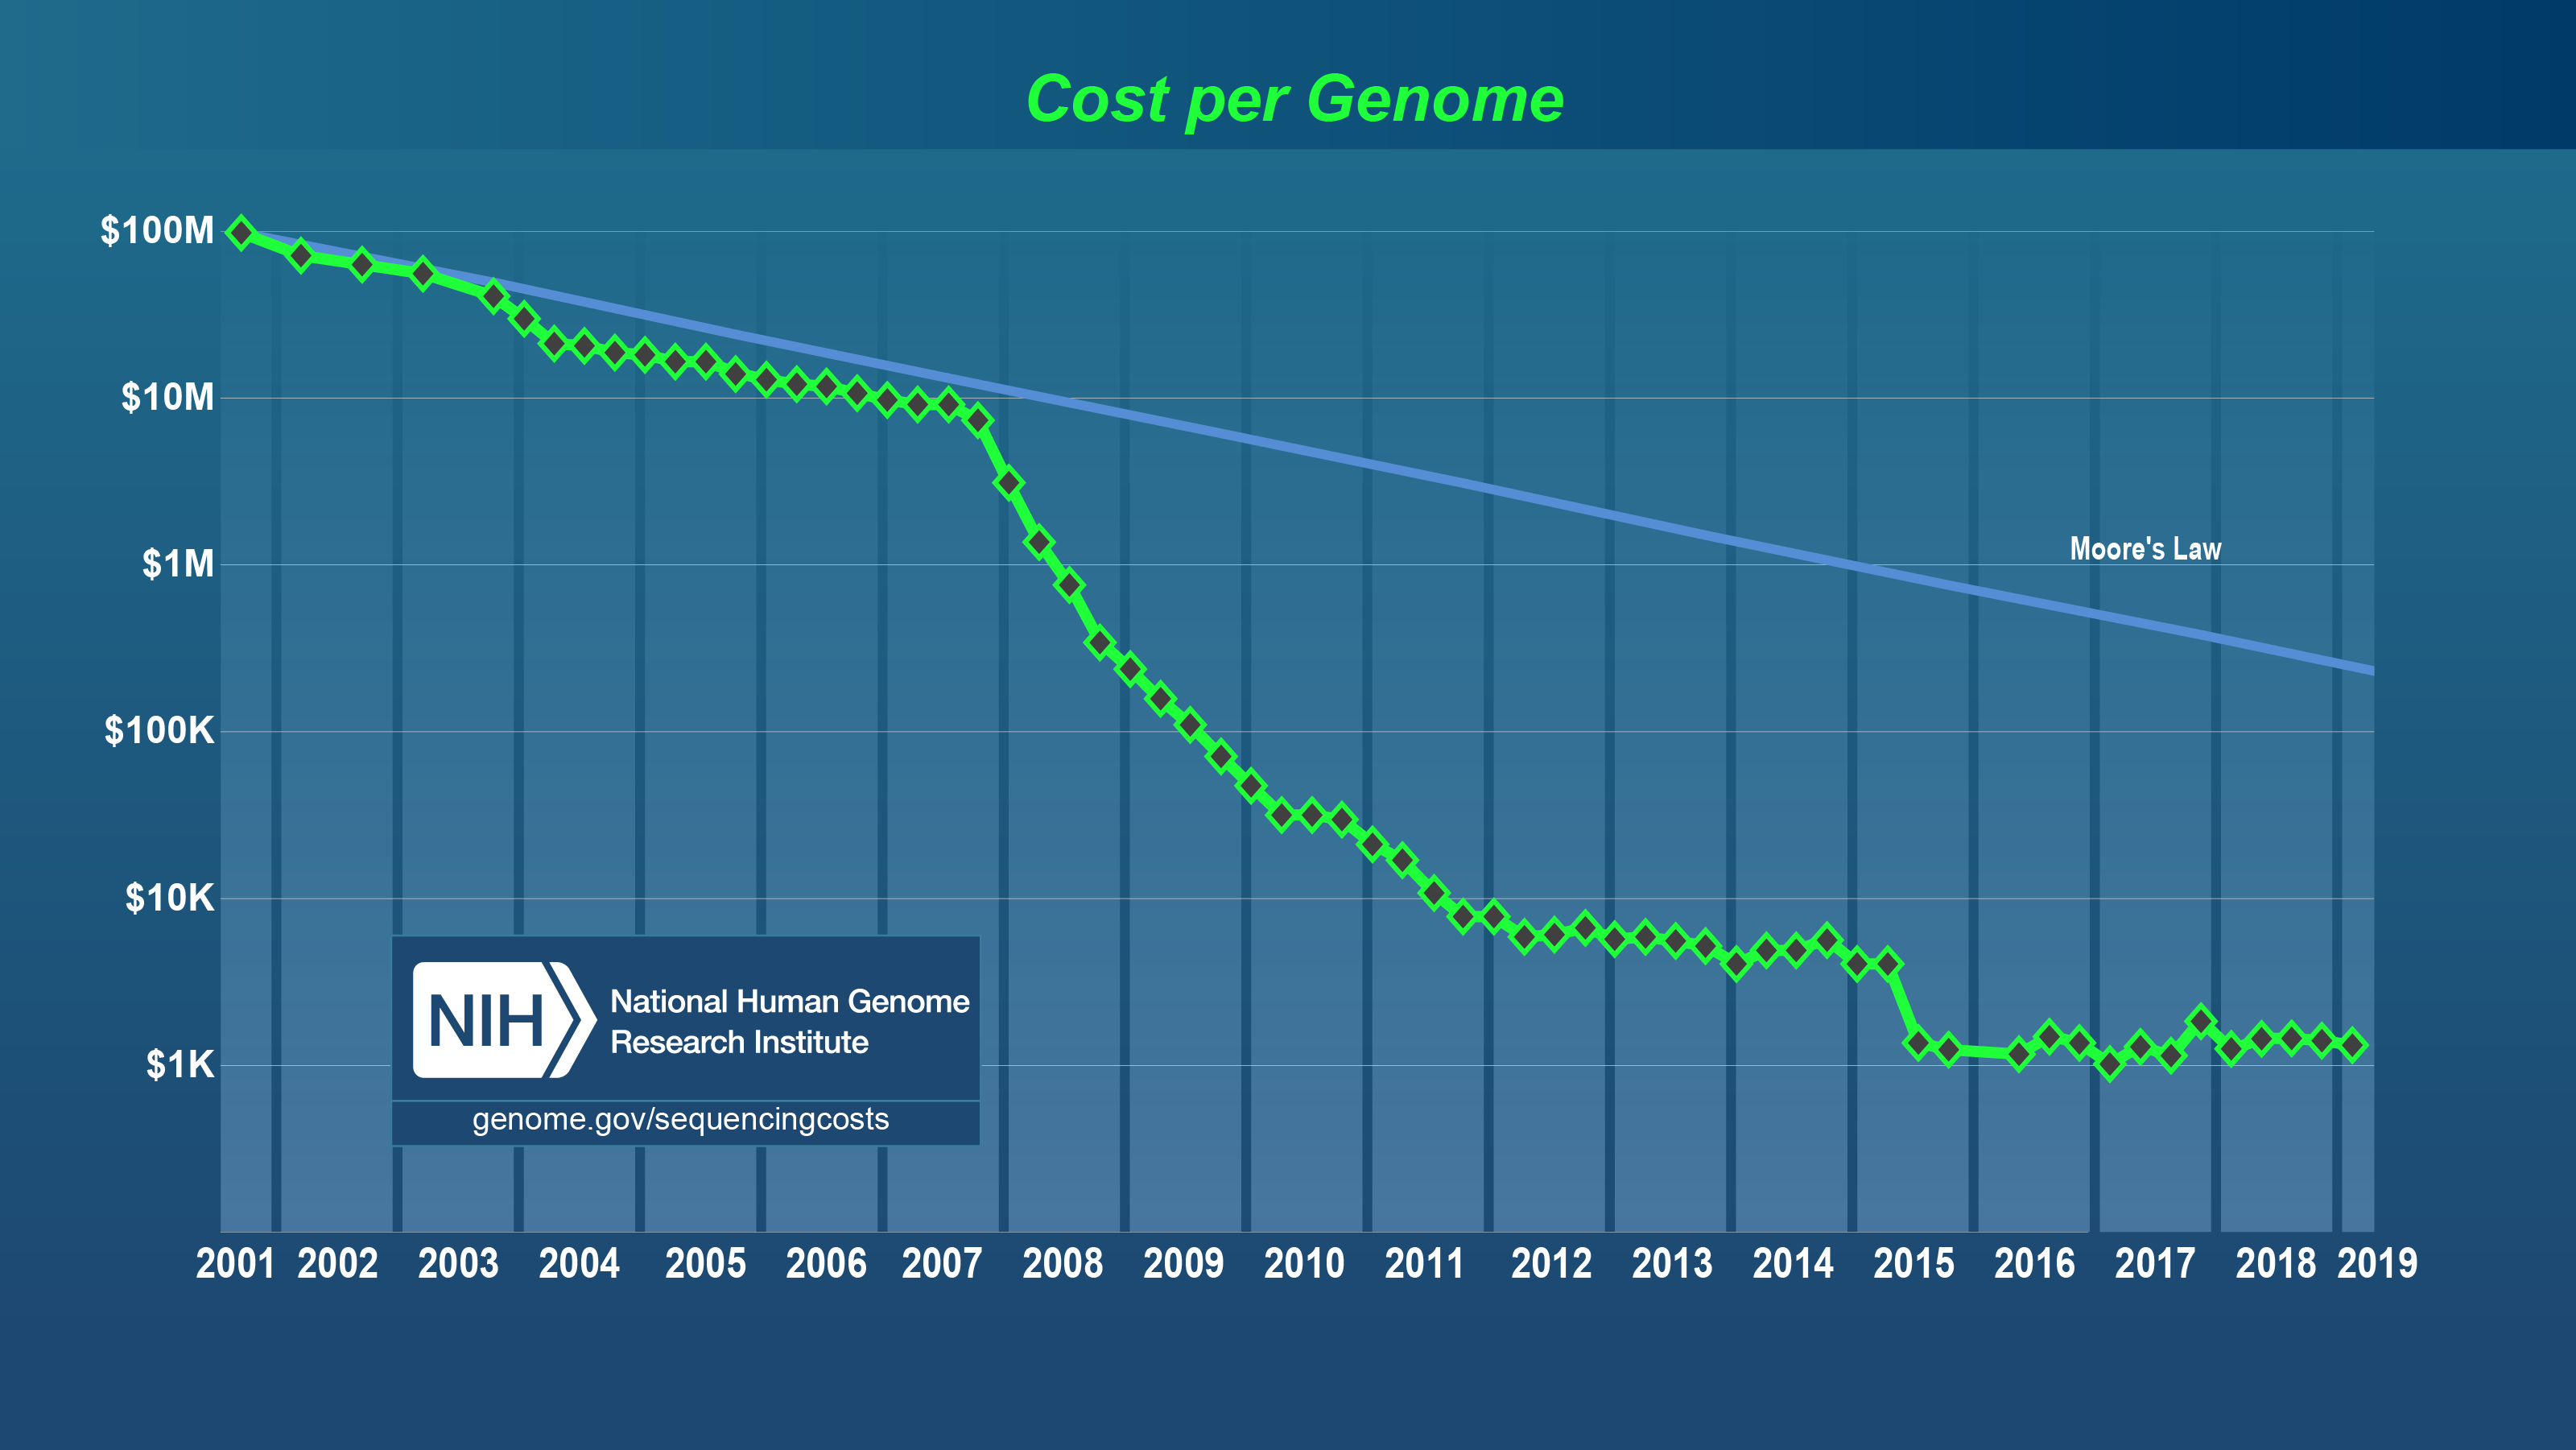
\includegraphics[width=300pt]{chapters/images/introduction/sequencing_cost_moore.png}
    \caption{The cost of sequencing a human-sized genome over time. Data from the NHGRI Genome Sequencing Program (GSP)~\cite{url-moore}.}\label{fig:seqcost}
\end{figure}

Shortly after the publication of the human genome, high-throughput RNA-seq techniques emerged to sequence the \emph{mRNA} molecules that are transcribed from the DNA, collectively termed the \emph{transcriptome}. This allowed for the identification and quantification of gene transcripts, providing valuable information about which genes are \emph{expressed} (active) at a given point in time, and at which levels. Furthermore, this also has the capability of providing researchers with information about post-transcriptional mutations and other complexities such as alternative splicing~\cite{wang2009rna}. Similarly, the study of epigenetics is revealing that non-coding DNA, far from the once-termed \textit{`junk DNA'}, is part of an intricate and complex regulatory system controlling the expression of genes~\cite{zuckerkandl2007combinatorial}.

Now we are moving into the era of \emph{third-generation} sequencing, where single-cell~\cite{gawad2016single}, long-read~\cite{koren2015one}, and often real-time sequencing~\cite{flusberg2010direct} are allowing for ever more accurate determination of nucleotide sequence, providing increased resolution even in highly diverse and complex samples such as cancer or metagenomic samples. All these technological advances have led to a deluge of data that must be managed and analysed, typically by bioinformaticians.


\section{The Bioinformatics Challenge}

With huge amounts of data now being generated at relatively low cost~\cite{chen2014big}, and compute resources being available even on moderate budgets, the challenge in genomic research has shifted from the sequencing technologies to the analysis and interpretation of these big and highly complex datasets, and the development of the software required in order to gain new understanding of the underlying biological systems. This poses significant challenges, both technologically and scientifically.


\subsection{A jigsaw genome}
Current sequencing techniques cannot simply read all the nucleotides of an entire chromosome at once; instead, DNA molecules are cut into tiny pieces of a few hundred bases, and each of those small fragments is then sequenced. The full genome must then be reconstructed from these short sequence reads. Think of this as solving a jigsaw puzzle with billions of pieces. To complicate matters further, the nucleotides determined by the sequencer (\emph{base calls}) are not always correct. Moreover, we typically don't sequence the DNA from just one cell, but combine material from a large number of cells together and leading to a lot of duplicate and overlapping pieces. And then of course, the genome itself contains complexities such as repetitive regions, that complicate the reconstruction further. Luckily however, in the case of human DNA, we have the picture on the puzzle box to guide us, in the form of the reference genome. This reference genome can be used as a scaffold to which to map each of the reads, improving our chances of successfully reconstructing the genome from the short read data. However, a reference genome does not exist for all organisms, and diseases such as cancer can incur high degrees of genomic rearrangements, decreasing the utitlity of the reference genome. In such cases, the short reads must be assembled \emph{de-novo} in order to reconstruct the genome.

\subsection{Ever-changing landscape}
Sequencing technologies are evolving at a staggering pace, and with them, so must the software tools capable of analysing the data. Therefore, new tools are developed continually and existing tools must be updated regularly to remain relevant. As a consequence, typically there simply is not enough time for community consensus and data and analysis standards to emerge organically before the advent of new technologies make them obsolete. Because of this, there usually are a multitude of tools available for any given task, each with their own set of advantages and disadvantages, and some of the main challenges are finding the right tool for the particular situation, and knowing when to use existing tools and when the development of novel tools is in order.


\subsection{Standardisation}
A typical bioinformatics analysis will consist of many different tools, chained together into a \emph{pipeline}. In order for data to pass smoothly from one tool to the next, it is important to agree on standard file formats. Unfortunately, in the absence of an authoritative body to prescribe such standards, these do not exist in many cases, and where they do, they often allow for a large degree of flexibility. As a result, files cannot always be passed seamlessly from one tool in the pipeline to the next, and custom file transformation steps are often required as a \emph{glue} of sorts between the different analysis steps.


\subsection{Data Storage}
 \begin{comment} https://qumulo.com/blog/genomic-sequencing-qf2-storage/ \end{comment}
It has been predicted that genomics may soon overtake other \emph{Big Data} domains such as astronomy and video-hosting platforms such as Youtube in terms of yearly data generation~\cite{Stephens2015}. Handling these vast amounts of data is a challenge many bioinformaticians face. Not only must the data be stored somewhere where it can be easily accessed, it must also be organised, backed up, and shared in an efficient way. Any storage solution must be able to scale to the exponential trend of growth both in size and number of files. Furthermore, data storage solutions must comply with privacy and security requirements, which is especially important in the case of human genetic data.


\subsection{The Specialist Bioinformatician}
All of these challenges have resulted in bioinformatics becoming a highly specialized field, which in itself poses a new challenge given the observation that the domain knowledge (biology) and the informatics know-how more and more often do not reside in a single individual, and the interpretation of the data cannot always be done by the person performing the data analysis and vice versa~\cite{preeyanon2014reproducible}. Instead, close communication between the two fields is required, and ideally the domain experts should be empowered to perform their own day-to-day data analyses without the need of a bioinformatician.


% some (partial) solutions to the above challenges, spoilers: open software, open science, open everything
\section{Bioinformatics Best Practices}

In order to optimally deal with all the challenges in bioinformatics, adhering to a set of best-practices guidelines may be beneficial. Such best practices have been described many times~\cite{sandve2013ten,Seemann2013,wilson2014best,prlic2012ten,altschul2013anatomy,via2013best,Leprevost2014}, with the most notable example being the widely-adopted FAIR (Findable, Accessible, Interoperable, Reusable) data principles~\cite{wilkinson2016fair}. The FAIR data project provides guidelines and tools to improve standardisation within bioinformatics.

\subsubsection{Findability}
The first step in (re)using scientific datasets, tools, or services, is to find them. Simply making these resources available online is not enough to make them truly findable. By annotating datasets and tools with metadata using standard ontologies allows them to be discovered more easily by both humans and computers. This will also allow services to be created to aggregate this information into discovery portals for users.


\subsubsection{Accessibility}
Accessibility of tools and data implies not only that these resources be made publicly available, but also that they are easily findable and \emph{usable}. Most bioinformatics tools are command line UNIX~\cite{url-unix} tools, and biologists are not typically trained in the use of such. Even for the experienced bioinformatician, running some of these tools can be a challenge due to lack of documentation or quality of the tool. Ideally, once a tool or pipeline has been validated, the analysis can be run by the domain expert, i.e.\ the research scientist responsible for the interpretation of the analysis results, without being reliant on the support of a bioinformatician at every step~\cite{kumar2007bioinformatics}.

Creating user-friendly software is not a trivial task. Application linking (also referred to as \emph{wrapping}), can ease this burden for the tool developer. In such an approach, existing user-friendly interfaces host third-party software packages --at minimum effort to the developer of the hosted software-- and thereby offer a layer of abstraction to the end-user that shields them from the implementation details of the tool and provides a uniform usage paradigm for all tools, regardless of their differences behind the scenes. Two examples of such hosting frameworks in the context of bioinformatics are Galaxy~\cite{giardine2005galaxy,goecks2010galaxy} and Taverna~\cite{oinn2004taverna}.

Accessibility also includes the creation of high-quality documentation of tools, both aimed at developers and end-users, and ideally some form of training manual to educate users in the proper use of tool and to warn about possible pitfalls and biases.

\subsubsection{Reproducibility}

A cornerstone of the scientific method is reproducibility of results. Experiments should be described in sufficient detail to allow for their reproduction and independent verification by fellow scientists. In theory, since bioinformatics occurs entirely in the digital realm --and is not dependent on physical samples as is in the wet lab-- it should be possible to completely reproduce an experiment provided that all the input data is available and the analysis is sufficiently well described. In reality however, this remains a big challenge, and many publications cannot be reliably reproduced based on the information provided therein~\cite{baggerly2009reproducible,kim2018reproducibility}.

As a result, reproducing bioinformatics analyses often becomes an exercise in \textit{forensic bioinformatics}; attempting to piece together the exact procedure used through trial-and-error and educated guessing, rather than by the information provided by the original researchers.
This is not without consequences; in some cases this has lead to clinical trials being started based on incorrect conclusions not revealed during peer review due to lack of reproducibility~\cite{baggerly2009reproducible}.

In recent years, many scientific journals have started taking steps towards remedying this situation, by improving submission guidelines for bioinformatics pipeline descriptions, similar to those they impose for the physical samples.
The latter are commonly required to be submitted to biobanks before submission, and the raw datasets generated from them to be stored in online repositories.
For true reproducibility of scientific findings, a standardised description of the full software stack used to analyse the data, as well as a detailed description of how this code was applied to the raw data in order to arrive at the presented conclusions must be provided.

\begin{comment}
Many journals require authors to submit datasets to public repositories in order to allow other scientists to reproduce their findings. With bioinformatics now such a fundamental part of any publication, a clear description of the analysis pipeline is also required for true reproducibility, but the majority of scientific publication do not contain all the information required to reproduce the in-silico experiment [cite]. Making analysis software open-source and adhering to a set of bioinformatics best-practices can improve the reproducibility of bioinformatics analysis pipelines.
\end{comment}

% dependency management
One obstacle to the reliable replication of bioinformatic studies arises from the fact that, while reproducibility is a high priority in the scientific community, this is not true for software developers in general, and bioinformatics pipelines are often dependent on a combination of scientific and more general-purpose components. For example, many software packages will simply be removed once an update has been made available, hindering scientific reproducibility of all but the most recent analyses. This is where package managers such as Conda~\cite{conda} or GNU Guix~\cite{courtes2013functional} and containner technologies such as Docker~\cite{url-docker} offer significant improvement, by allowing any historic versions of tools to be installed at all times~\cite{kulkarni2018reproducible}. This aims to ensure that the full stack of software and dependencies obtained during installation of the pipeline will yield identical results when performed today as it will a year or 5 years from now.

% provenance
However, in addition to describing the complete software stack used for analysis, the pipeline \emph{provenance} must also be captured; metadata describing \emph{how} the tools were applied to the data in the analysis run. This includes the sequence and interplay of different tool executions, with the full set of parameters, and the input and reference data used at every step. Keeping a lab journal of the in-silico experiment is a good start, but is too error-prone as a manual process. Projects such as Jupyter Notebooks~\cite{kluyver2016jupyter} for Python, or Sweave~\cite{leisch2002sweave} and KnitR~\cite{xie2014knitr} for R, allow for the intermixing of text and code to create a kind of interactive journal article. Calculations can be embedded within the text, and these calculations may be examined and rerun or adjusted with ease by the reader. A drawback of this approach comes when tools require a lot of resources or are not all written in the same language, as is typically the case for bioinformatics analyses. Workflow platforms such as Galaxy automatically keep track of provenance for the user and have the advantage of supporting a wide range of tools and programming languages.

\begin{comment}
``forensic bioinformatics'' -> have to figure out by trial and error what was done

https://bmcmedresmethodol.biomedcentral.com/articles/10.1186/s12874-017-0377-6
https://www.biostars.org/p/52561/
https://www.nature.com/naturejobs/science/articles/10.1038/nj7396-137a
https://www.nature.com/nm/journal/v13/n11/full/nm1107-1276b.html
\end{comment}

\subsection{Interoperability}

% standards
The aforementioned lack of data format standards hinders the interoperability of tools. Even in cases where file formats are somewhat standardized, variations in the exact implementations may still require careful consideration within a pipeline. Consider for example the FASTQ format; this is a widely used and relatively simple format, it consists of 4 lines per sequence read, but the line containing quality score, is the source of some divergence in the format. Different tools and sequencing platforms use different encoding schemes, but this information is not stored within the file itself, making it hard to ascertain which encoding scheme was used without proper metadata accompanying the file. Knowing the quality encoding scheme used for any datasets entering your pipeline is of critical importance, as low-quality reads could be mistaken for high-quality reads and vice versa if incorrect assumptions are made. Similar widespread variations in standard formats include chromosomal location (0-based or 1-based numbering, open or closed) and chromosome names (with or without a \verb+chr+ prefix) or gene names (many different naming schemes). These issues are not hard to deal with on a conceptual level, but in practise can easily lead to inaccurate results if not carefully taken into account by the creator of the pipeline.

Such concerns exist on the more purely informatics side of bioinformatics as well. Take the example of command line shell scripts, many OS-dependent syntax variations can hinder interoperability, but by taking care to comply with POSIX standards~\cite{walli1995posix}, such concerns can be mitigated.

% technical interoperability
Going beyond file formats, interoperability of different tools may be hindered due to the fact that they are often written in different programming languages and/or designed for different operating systems. Fortunately, tool developers can undertake steps to make their tools more interoperable. Package managers such as Bioconda~\cite{gruning2017bioconda} will compile software from its source for a variety of different operating systems and simplify installation for end users.

% documentation!
Finally, and vitally, precise documentation of any assumptions made in the code is indispensable, and making source code open further facilitates this transparency and interoperability~\cite{ince2012case}.


\subsection{Maintainability}
Since scientific research depends increasingly on software, decreasing the burden of tool maintenance is valuable and worthwhile pursuit. Furthermore, many tools are written by small research groups or single individuals who are simply unable to perform the necessary maintenance without support. By making tools open-source, the entire bioinformatics community is able to step up as co-developers, allowing them to discover bugs and contribute fixes or enhancements. Code sharing platforms like GitHub~\cite{url-github} and BitBucket~\cite{url-bitbucket} facilitate this community-driven approach to software maintenance.

Using code versioning such frameworks such as git~\cite{url-git} or mercurial~\cite{url-mercurial} ensures precise tracking of changes and enable collaborative tool development. Incorporating tests at every phase of development can further decrease the maintenance effort. Unit tests ensure that small code modules show expected behaviour at all times. Functional tests ensure that these different units of code always yield the desired result when working in conjunction. Code quality checks can help streamline the code itself and increase readability, benefiting future development. Continuous integration is the paradigm whereby changes to the mainline code are incorporated incrementally and continually, and thoroughly reviewed and tested at every stage, thereby decreasing the maintenance burden of the software. Code sharing platform such as GitHub and BitBucket offer continuous integration frameworks as part of their service.



\section{Bioinformatics for Everybody}

In order to make bioinformatics accessible to a wider audience, and empower domain experts to analyze their own data, several components are required. Firstly, analyses must be made available in a user-friendly way, not requiring any expertise in programming or systems administration to install and run the pipelines. Secondly, data visualisation and integration are essential components to aid the interpretation of results by the research scientist in this \emph{big data} era. Finally, extensive training of researchers is crucial in order to provide them with the required knowledge and confidence to run analyses and interpret outcomes independently.

\subsection{The Galaxy Project}
The Galaxy project~\cite{afgan2016galaxy} provides a user-friendly graphical interface to command line tools, bringing the data analysis to the domain experts equipped to perform the interpretation of the results. It also facilitates many of the best-practice bioinformatics guidelines outlined in the previous section; with its heavy focus on accessibility and reproducibility, Galaxy is a potent framework for creating high-quality bioinformatics pipelines. Galaxy keeps track of the full analysis provenance, manages tool dependencies with Bioconda~\cite{gruning2017bioconda}, has built-in visualisations, and is accessible by end users with nothing more than a web browser. For developers, Galaxy provides a convenient framework to package tools to make these available for researchers throughout the global community. The Galaxy tool shed~\cite{url-toolshed} is the central repository of tools that anybody may contribute to, and contains over 7200 tools at the time of this writing. As such, it is a powerful resource for making bioinformatics accessible and reproducible.

\subsection{Visualisation and Reporting}
As scientists become increasingly reliant on large and complex computational analyses in their research~\cite{chen2014big}, the final analysis result datasets become similarly complex and have often grown beyond the realm of what can be manually viewed and interpreted, both in terms of the number of files and their sizes, as in terms of complexity. Analysis results therefore require summation and visualisation and must be presented to the domain expert in a comprehensible and accessible manner. Such a report should also contain detailed descriptions of the methods used and assumptions made and citations to any third-party tools employed, as an understanding of these factor can assist in interpretation~\cite{kumar2007bioinformatics}.

For genomics data, visualisation tools such as Circos~\cite{circos} and MultiQC~\cite{ewels2016multiqc} enable the integration of various output datasets, often in the order of millions of lines each, to be summarized in a single image or report. While some resolution may be lost in such visualisations, they do enable the easy identification of areas of interest and guide the interpretation by pointing the domain experts in the direction of further inspection.


\subsection{Training}
With -omics research becoming increasingly computational in nature, and many research groups not having access to enough dedicated bioinformaticians, there is a great need for high-quality bioinformatics training to ensure that the domain experts who interpret the results of data analyses are optimally equipped to do so. Surveys confirm this need for bioinformatic training; the majority of researchers (>95\%) work with or plan to work with large datasets, but most (>65\%) possess only minimal bioinformatics skills and are not comfortable with statistical analyses~\cite{larcombe2017elixir,williams2017vision}. Demand for training currently greatly exceeds the supply~\cite{attwood2017global}. In a recent survey~\cite{survey2013embl} over 60\% of biologists expressed a need for more training while only 5\% called for more computing power. This indicates that the true bottleneck of the current data deluge is not storage or processing power, but rather the knowledge and skills to utilize existing resources.

With its focus on accessibility and user-friendliness, the Galaxy platform is not only a great workflow management system, but also an ideal environment for teaching. Trainees are shielded from the minutiae of the implementation details of the underlying tools, and need nothing more than a browser to execute the tutorials. Because Galaxy can host any command line tools and the tools available in the tool shed cover a wide range of topics, creation and maintenance of a set of training materials must be a collaborative community effort, with content being created by a large number of people with expertise in the various topics.

\subsection{Bioinformatics in the Clinic}

With the decreasing costs of next-generation sequencing, and the increased accessibility of the tools and compute resources required for analysis, bioinformatics is increasingly being incorporated directly into the clinic. In contrast to research applications, clinical bioinformatics directly informs disease management and patient care.
Therefore, careful validation of all tools and pipelines is required to ensure quality of the results. Furthermore, there is great need for standardisation of pipelines to ensure a uniform standard of care across clinics. Finally, there is a greater need for data security and privacy as compared to research applications, as clinical data usually involves patient identifiable data.
To this end, a set of 17 best-practice recommendations for the validation of clinical NGS-based bioinformatics pipelines have recently been published by the Association of Molecular Pathology (with support from the College of American Pathologists and the American Medical Informatics Association)~\cite{roy2018standards}.
While these recommendations focus on variant analysis, most guidelines are applicable more broadly. These guidelines include practical recommendations for the design, development, and operation of the analysis pipelines, with an additional emphasis on the importance of properly trained and qualified molecular professionals.
These clinical guidelines recommend that laboratories perform their own validation, led by a medical professional well-trained in NGS interpretation. The validation process should closely mimic the real-world scenarios faced by the lab. Validation should occur both on each component of the bioinformatics pipeline individually, as well as the full end-to-end functionality of the pipeline as a whole.
Additionally, the set of QC metrics employed to determine the performance of the pipeline must be evaluated as part of the validation process.
Furthermore, since there is a general lack of standardization in bioinformatics, clinical validation must specify and ensure standardization of nomenclature throughout the pipeline. This entire process of validation must be repeated whenever any component in the pipeline is altered.
Furthermore, validation must ensure that pipelines are compliant with any applicable lab accreditation standards, as well as comply with the relevant laws concerning data security with regards to patient identifiable data.
Moreover, clinicians must be alerted to any unintended or unauthorized changes to data files.


Many of these recommendations have significant overlap with general bioinformatics best-practice guidelines.
For example, bioinformatics best-practices call for extensive code review and unit- and functional testing, as well as continuous-integration testing, standardisation of file formats and nomenclature, and data security and integrity checks.
By adhering to these bioinformatics guidelines from day one of development of any tools and pipelines, we ease the burden of clinical validation, and increase the likelihood of adoption of tools and pipelines within the clinic.
%Furthermore, the need for training of medical professionals in NGS interpretation cannot be understated.

\subsubsection{Data protection}
In clinical bioinformatics, data are typically pseudo-anonymised before analysis, decoupling the sequencing data from the clinical metadata, and assigning an anonymous identifier for the sample. This allows the sequencing data to be analyzed externally, while the clinical data resides in separate data repositories such as OpenClinica~\cite{cavelaars2015openclinica}, only accessible to a limited number of clinicians directly involved in the patient's care. However, as sequencing techniques become more accurate, and our knowledge of the relationship between genotype and phenotype increases, privacy concerns also grow, and we must be continually re-evaluate the security risks and their mitigations when dealing with NGS data~\cite{erlich2014routes}.

\subsection{Use Cases}
The following sections describe the two real-world research areas where bioinformatics is of great importance; cancer genomics and clinical microbiota profiling. In both examples, implementation of the bioinformatics concepts and best practices described above provide valuable benefits to the research scientists.


% Use case 1: Prostate Cancer

\newpage
%\cleartoleftpage
\thispagestyle{empty}
\begin{center}
\vspace{2cm}
\begin{minipage}{5in}
\tikz[remember picture,overlay]
\node[opacity=0.8,inner sep=0pt] at (current page.center){
\includegraphics[width=\paperwidth,height=\paperheight]{frontmatter/images/border-1.png}};

\begin{center}

{\Large The Jigsaw Genome \normalsize
\vspace{2cm}


I like puzzles. Any type of puzzle. I always have. If I see a puzzle or a problem I have to solve it. I think that is what makes cancer such a fascinating topic for me.

\vspace*{0.5cm}

Imagine you are given a jigsaw puzzle. Now instead of a few hundred pieces, there are several billion pieces. The picture on the box is not a picture of the puzzle inside the box, it is just a somewhat similar image. Oh, and did I mention there are a whole bunch of pieces missing? And that many pieces are duplicated? Some pieces don't even belong in our box, but come from a completely different puzzle. On top of that, your little sister has spilled paint over some of the pieces so those can't be trusted to reliably contribute to the image. And instead of one single puzzle, the box contains several; they are all variations of the image on the box, but you have no idea how many different puzzles the box contains. Sound challenging? This is the problem we are solving whenever we sequence a cancer genome.

\vspace*{0.5cm}
\textbf{[Metaphor key]} \\
\textit{puzzle pieces} = sequence reads \\
\textit{picture on box} = reference genome \\
\textit{missing pieces} = hard-to-sequence areas \\
\textit{other puzzles} = contamination \\
\textit{painted pieces} = sequencing errors \\
\textit{multiple puzzles in box} = clonality
}

\end{center}
\end{minipage}
\end{center}



\newpage
\section{Use case 1: Prostate Cancer}

\epigraph{3in}{The time has come in America when the same kind of concentrated effort that split the atom and took man to the moon should be turned toward conquering this dread disease.}{President Richard Nixon}

On December 23, 1971, President Richard Nixon, buoyed by recent technical feats such as the moon landing, signed into law the National Cancer Act, thereby declaring a war on cancer. Today, more than 45 years later, that war is still being waged in full force. While great advancements have been made towards this goal, some of the initial optimism has been quelled by discoveries of the great complexity and heterogeneity underlying cancer.


\subsection{The Hallmarks of Cancer}

Tumor cells evolve from normal cells through the acquisition and accumulation of mutations.
The human body has mechanisms in place to repair or dispose of damaged cells and to prevent runaway cell division, so in order for a tumour cell to survive and thrive it needs to acquire changes that provide it with advantages for proliferation and evasion of the cell's defense mechanisms.
Evidence suggests this transformation from healthy cells into malignant cells follows a strikingly similar path across all different tumour types~\cite{hanahan2000hallmarks}.
A cell's acquired abilities that drive tumour progression are known as the \emph{hallmarks of cancer}~\cite{hanahan2000hallmarks,hanahan2011hallmarks,lazebnik2010hallmarks,horne2015evolutionary,fouad2017revisiting} and includes such traits as evasion of immune response and programmed cell death, self-sufficiency in growth signals and insensitivity to anti-growth signals, limitless replicative potential, sustained angiogenesis (creation of new blood vessels), tissue invasion and metastasis, reprogramming of energy metabolism, genome instability, and tumor-promoting inflammation.

Each of these steps overcomes one of the body's anti-cancer defense mechanisms. This evolution into malignancy is an Darwinian process where the mutations acquired are random, but those cells that have gained mutations which are advantageous for survival will be able to replicate and thrive and accumulate further mutations. Distinguishing the mutations that impart a strategic advantage and thereby \emph{drive} a tumour's progression, from the often huge number of less harmful \emph{passenger} mutations accumulated over the lifetime of a cancer cell is crucial to our understanding of cancer progression~\cite{stratton2009cancer}. The optimal course of treatment for a patient often depends on the mutations present and how the cell functions are subsequently impacted by those mutations. %However, many different mutations may lead to the same disruptions of key pathways, therefore we must evaluate mutations not just at the DNA level but in the broader context of their functional impact on the cell's internal processes.



\subsection{Cancer's Complexities}

Determining the exact genetic sequence of healthy individuals is already quite a challenging endeavor; trying to extend this to cancer genomes takes this challenge to the extreme. There are several complexities present in cancer genomes that make accurate determination of the genetic changes and their downstream impacts a difficult task. In the following sections we will discuss some of these complexities and explore the informatics challenges they pose.

\subsubsection{The Bio}

\paragraph{Small variants} comprise the simplest class of mutations; those consisting of alterations of just a handful of bases, for instance the \emph{substitution}, \emph{deletion} or \emph{insertion} of one or more nucleotides.

The impact of such mutations depends on where in the genome they occur. Single nucleotide variants (SNVs) in exonic regions can range from having no effect on the resulting protein (silent), to changing an amino acid in the protein to a different amino acid (missense mutations), to changing a codon into a stop codon (nonsense mutation), which nearly always results in a nonfunctional protein. If this happens in a protein that is vital to the functioning of the cell this can lead to a range of health conditions~\cite{cargill1999characterization}.

While variants within the coding sequence are most likely to have an impact on cell health, small variants \emph{outside} the coding sequence can also have drastic impact on health~\cite{zhang2015non}. For example, 70\% of melanomas exhibit a point mutation in one of two positions in the promoter region of \emph{TERT}~\cite{horn2013tert,huang2013highly}, suggesting such somatic point mutations in regulatory regions may play a role in tumorigenesis. Therefore, whole-genome sequencing may reveal valuable information not detected using exome sequencing.


\paragraph{Structural Variants (SVs)} are larger-scale mutations involving rearrangement of segments of DNA of more than roughly 50 bp. In some cases, these rearrangements can cause (parts of) two genes that are usually separated by some distance on the genome to come together to form new hybrid genes. In some cases, these fusion genes may be transcribed into fusion proteins, with a potentially disruptive effect on cell processes. The text book example of such a gene fusion is the so-called Philadelphia fusion frequently observed in leukemia~\cite{de1982cellular,heisterkamp1990acute}. In this Philadelphia chromosome, a translocation between chromosomes 9 and 22 leads to a fusion of the \emph{BCR} and \emph{ABL1} genes. This fusion gene is expressed, and the aberrant fusion protein causes disruptions to key signalling pathways governing the cell cycle, causing the cells to divide uncontrollably and thereby drive tumor progression. Accurate detection of such structural variations is crucial, as they may serve as diagnostic markers~\cite{nowell1960chromosome,nowell1961chromosome} or even therapeutic targets~\cite{druker2001activity,druker2001efficacy}.

SVs most often occur outside coding regions, but this does not diminish their capacity for great impact, for instance by disruption of the regulatory mechanisms of tumour suppressor genes or oncogenes~\cite{yi2018patterns}. These types of SVs not involving coding regions directly, may only be detected through whole-genome sequencing using paired-end sequencing. In rare cases, a phenomenon known as \emph{chromothripsis} may occur. In contrast to the more common gradual acquisition of mutations over time, chromothripsis involves a shattering of (part of) a chromosome in a single catastrophic event, and the subsequent imprecise stitching back together of the genetic sequence by the cell's repair mechanisms. This results in a cluster of thousands of SVs in a confined genomic region. Chromothripsis occurs in about approximately 2\%-3\% of cancer genomes, with a significantly increased rate incidence in some cancer types~\cite{luijten2018}. Identification and reconstruction of such highly rearranged cancer genomes in order to predict their effects remains an open challenge~\cite{yang2016chromothripsis,govind2014}.

% TODO: mention paired-end sequencing for SV detection?

% good review paper for chromothripsis: luijten2018

%Numerous fusion genes have been found to play a role in tumorigenesis~\cite{TODO},
%in prostate cancer the TMPRSS2-ERG fusion is present in roughly 40\% of tumours,~\cite{TODO}


\end{justify}

\paragraph{Tumor heterogeneity} refers to the phenomenon that cells in different physical areas in a tumour may be genetically very distinct. When a tumour cell divides to create two new cells, these daughter cells will acquire new mutations.

\begin{wrapfigure}{r}{0.5\textwidth}
%\begin{figure}[h!]
    \centering
    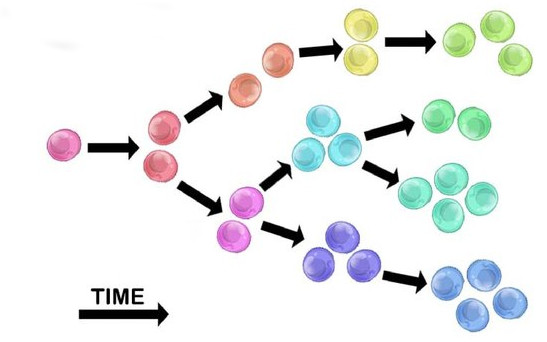
\includegraphics[width=0.4\textwidth]{chapters/images/introduction/heterogeneity.jpg}

    \caption{As tumour cells divide, they may acquire additional mutations. Different areas of the tumour may follow different evolutionary paths, leading to tumour heterogeneity.}
    \label{fig:heterogeneity}
%\end{figure}
\end{wrapfigure}

%image from wiki commons: https://en.wikipedia.org/wiki/Tumour_heterogeneity#Clonal_evolution


Over time, this may lead to the formation of different clusters of cells each with a different set of acquired mutations. As a cell obtains a mutation that is beneficial to proliferation, it may instigate a new cluster, or \textit{clone}, of genetically similar cells while in other areas of the tumour, cells may follow a different evolutionary path and create genetically different sub-clones (Figure~\ref{fig:heterogeneity})~\cite{swanton2012intratumor}.

When sequencing a tumour, DNA from different cells --and thus potentially very different genomes-- is mixed together and sequenced as one. Reconstructing the different clonal genomes from this data is immensely challenging.


\paragraph{Further complexities} in the analysis of cancer genomes include the temporally evolving nature of tumours; performing the same sequencing experiment on the same tumour at different points in time will often yield a very different picture as the composition of the tumour and the acquired mutations will have changed. This further complicates the process of comparing different samples and elucidating key characteristics that have the potential to aid in the diagnosis and treatment of patients. Furthermore, studies in epigenetics have shown that tumorigenesis is not solely driven by mutations in nucleotide sequence, but secondary alterations such as DNA methylation may have an equal if not greater impact~\cite{pacchierotti2015environmental}.

\begin{justify}

\subsubsection{The Informatics}

All these complexities in the biology of cancer genomes translate to complexities of the downstream informatics analysis pipelines.

Mutations in DNA are described relative to a \emph{reference genome}, and comparing variants across different samples is inherently challenging for a variety of reasons. Observed differences between a sample and the reference genome could indicate a true biological variant, or be the result of a sequencing or mapping error, and separating the true variants from the noise is a task that each variant calling tool approaches differently. As a result, different variant callers often have poor overlap~\cite{orawe2013, hwang2015systematic}. This poor concordance combined with the observation that there often exist multiple different yet equivalent ways of describing a variant (Figure~\ref{fig:variant-multiple-representations}), which hinders the comparison of variants between different samples and studies~\cite{zook2014integrating}.

\begin{figure}[h!]
    \centering
    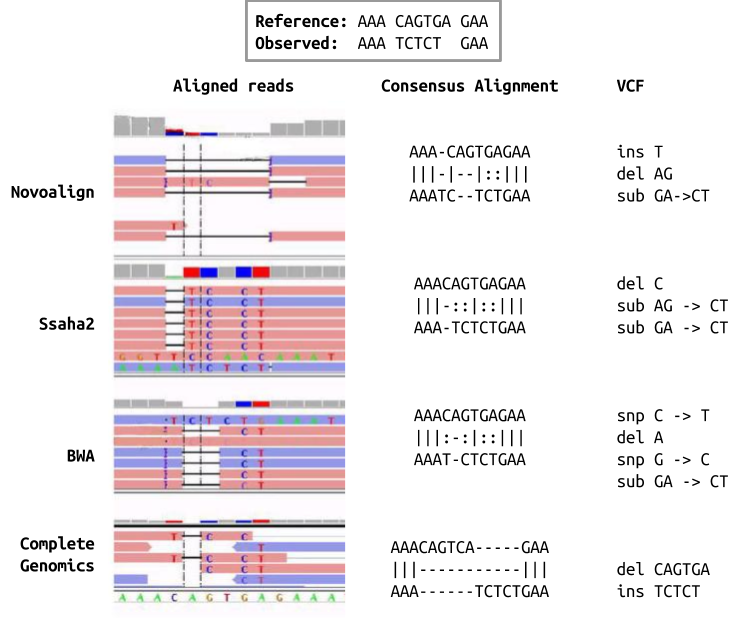
\includegraphics[width=0.5\textwidth]{chapters/images/variant-representation-all.png}
    \begin{comment}
        image in google drive https://docs.google.com/drawings/d/1WWmzW6uWtJ7HZ5WVgtg_oAMA_3E_569M4Ikjz4Ecjic/edit
    \end{comment}
    \caption{Complex variants can be represented in multiple ways. Four different aligners (Novoalign, Ssaha2, BWA, Complete Genomics) treat the same variant in vastly different ways, which leads to such differing sets of variant descriptions in the VCF files that it is no longer apparent that these variants in fact describe the same observed sequence. Image adapted from the Genome in a Bottle Consortium~\cite{zook2014integrating}.}
    \label{fig:variant-multiple-representations}
\end{figure}


%In the case of many tumour genomes, the high rate of mutations combined with possible high clonality and polyploidy generate further noise and complexity impeding the accurate determination of variants.
In cancer studies often aim to distinguish the \emph{somatic} mutations --those acquired by the cells during tumorigenesis-- from the individual's \emph{germline} variants that are present in every cell. To this end, normal tissue is often sequenced alongside the tumour material, and the resulting variant sets are compared to elucidate the set of mutations only present in the cancerous DNA\@. Therefore, having accurate variant callers and intelligent methods of variant comparison is of vital importance. However, even methods designed specifically for the identification of somatic variants~\cite{xu2014comparison,kim2013comparing,roberts2013comparative} show poor agreement~\cite{alioto2015comprehensive, kroigaard2016evaluation, orawe2013}, and improvements are continually sought~\cite{callari2017,vijayan2017}.

Structural variations are by definition large-scale variants, and most sequencers use short reads, making SVs dificult to detect. Consequently, the concordance between different SV calling methods is even poorer than for the small variants~\cite{sedlazeck2017}. This issue is compounded by a lack of a standard file format~\cite{scherer2007} making comparisons between studies very difficult. The advent of third generation (long-read) sequencing offers prospects of improving SV detection~\cite{sedlazeck2018,merker2017}. These methods typically have higher error rates than short read sequencing techniques, but by using a hybrid approach the advantages of long read sequencing can be combined with the accuracy of short reads to optimize detection of large scale genomics rearrangements~\cite{fan2017hysa,weissensteiner2017, miller2017, ritz2014}.

\newpage
%\cleartoleftpage
\thispagestyle{empty}
\begin{center}
\vspace{2cm}
\begin{minipage}{5in}
\tikz[remember picture,overlay]
\node[opacity=0.7,inner sep=0pt] at (current page.center){
\includegraphics[width=\paperwidth,height=\paperheight]{frontmatter/images/border-2.png}};

\begin{center}

{\Large The Human Microbiome \normalsize
\vspace{1cm}


\epigraph{5in}{\normalsize ``By the means of Telescopes, there is nothing so far distant but may be represented to our view; and by the help of Microscopes, there is nothing so small as to escape our inquiry; hence there is a new visible World discovered to the understanding. By this means the Heavens are open’d and a vast number of new Stars and new Motions, and new Productions appear in them, to which all the ancient Astronomers were utterly strangers. By this the Earth it self, which lyes so neer to us, under our feet, shews quite a new thing to us, and in every little particle of its matter, we now behold almost as great a variety of Creatures, as we were able before to reckon up in the whole Universe itself.''}{Robert Hooke, 1665 (in the Preface of Micrographia)}



\vspace*{1cm}
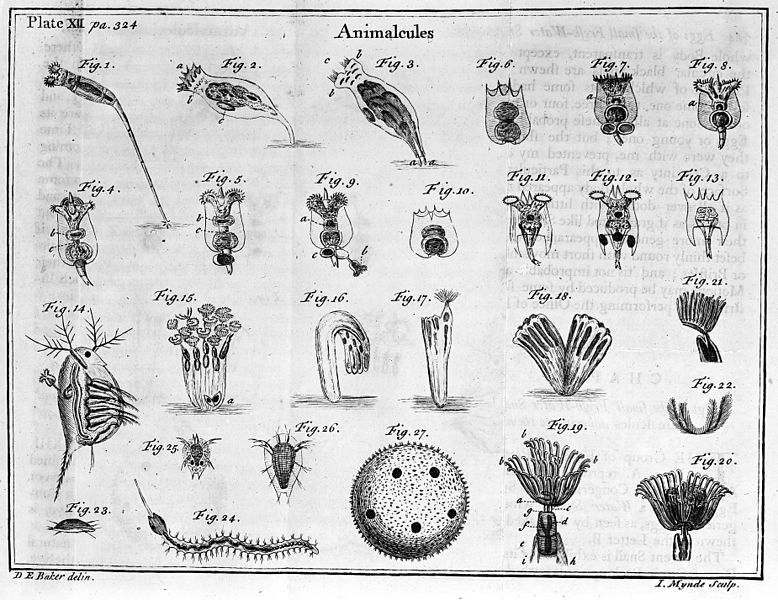
\includegraphics[scale=1.75]{chapters/images/mycrobiota/animalcules2.png}

}

\end{center}
\end{minipage}
\end{center}

\newpage


\section{Use case 2: Microbiota profiling}

\begin{comment}

overview of reading materials about the human microbiome

http://www.richardsprague.com/note/2017/10/16/best-academic-papers-about-the-microbiome/

informal history of microbiology: https://www.bioexplorer.net/history_of_biology/microbiology/
\end{comment}


In 1682, Dutch inventor and scientist Antonie van Leeuwenhoek first turned his microscope to a drop of rain water and discovered within a wealth of microscopic life which he termed \textit{animalcules}. With this finding, a whole new world of knowledge opened up, as it became clear that while these organisms might be microscopic in size, their capability to impact on human lives was enormous, causing food spoilage and disease. Through continued study over the following centuries, links between particular microorganisms and disease were discovered, and remedies developed.

More recently, researchers have realised the importance of not only studying the relationship between specific microorganisms and disease, but also of the structure and composition of the human microbiome \emph{as a whole} with respect to human health. This observation has led to the launch of large-scale research efforts such as the Human Microbiome Project~\cite{turnbaugh2007human} and MetaHIT~\cite{ehrlich2011metahit} to investigate the links between the microbiome and health, and kickstarted a wealth of new research.


\subsection{The Bio}

Every cell in our body contains a copy of our genome in its nucleus, which has been dubbed the blueprint of life. But these cells are not the only source of genetic material in our bodies; each one of us harbour a vast amount of micro-organisms at various anatomical locations. %(Figure~\ref{fig:microbiome});.
Estimates put the number of microbial cells as equal to or outnumbering human cells~\cite{sender2016outnumbered}. These microorganisms influence our metabolism, impact our health and immunity, and may affect drug efficacy. If our genomes are the blueprint of life, then our microbiomes are an important overlay to this blueprint; or, when we consider the genome as the \emph{source code} of life, the microbiome is an essential \emph{third-party plugin}. For this reason, the microbiome is often referred to as our \emph{second genome}~\cite{grice2012microbiome}, and has emerged in recent years as an important field of biomedical study. Links between the microbiome composition and diseases have been demonstrated in a number of diseases~\cite{cho2012human} including psoriasis~\cite{gao2008substantial}, obesity~\cite{turnbaugh2006obesity, ley2005obesity}, and colorectal cancer~\cite{castellarin2012fusobacterium,kostic2012genomic}, though in many cases a causal link remains to be proven.

\begin{comment}
\begin{figure}[h!]
    \centering
    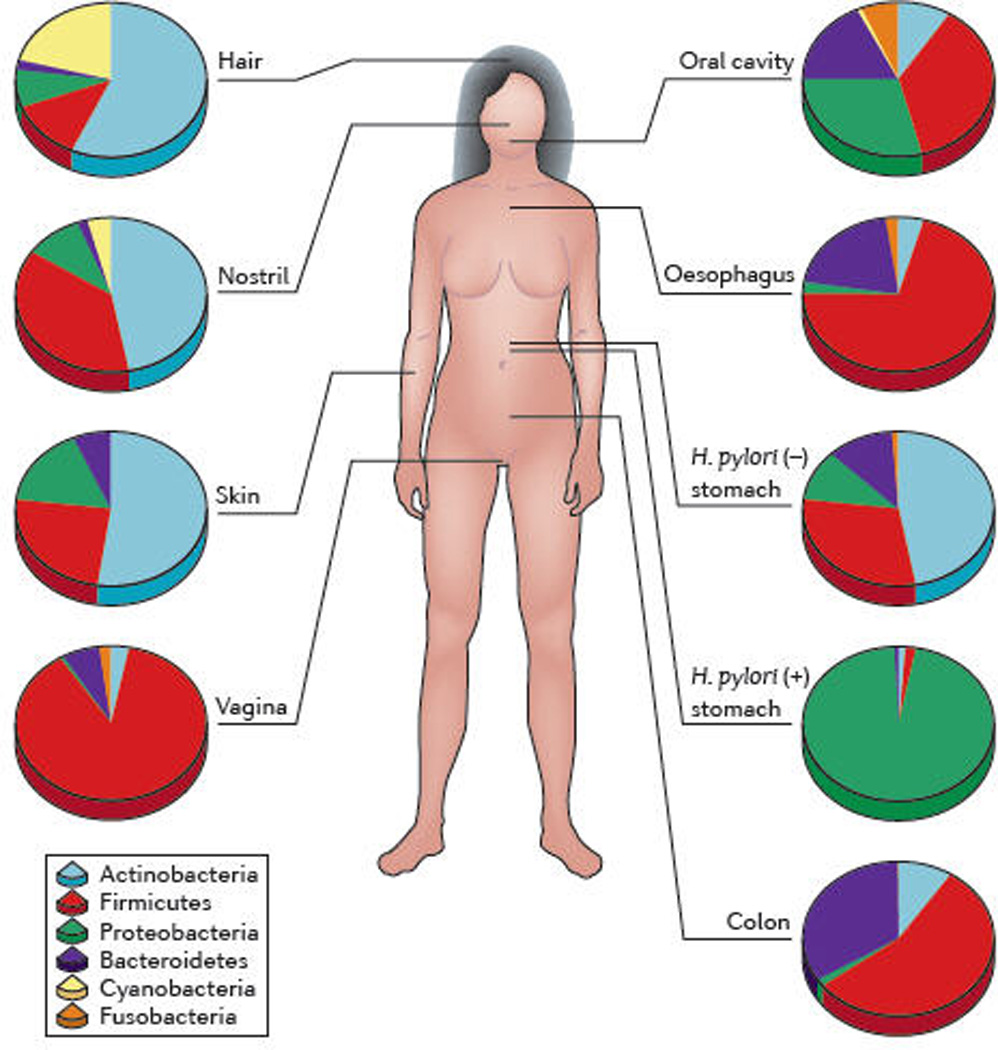
\includegraphics[width=250pt]{chapters/images/mycrobiota/microbiome.jpg}
    \caption{Presence of microbiota at different anatomical site in the human body and in different compositions}
    \label{fig:microbiome}
\end{figure}
\end{comment}



\subsection{The Informatics}

Sequencing the human microbiome comes with its own unique set of challenges. Because the microbiome typically consists of a large number of different organisms, this situation is akin to solving hundreds or thousands of jigsaw puzzles simultaneously, with all the pieces mixed together in a single box. Depending on the research objective, different approaches may be used to sequence the microbiome. Amplicon sequencing is a targeted approach where a (part of a) single gene is sequenced, which is sufficient for taxonomic identification of the organisms in the sample. In order to obtain additional information about the functional profile of the organisms in the community (for example screening for antibiotic resistance genes), whole-genome \emph{shotgun} sequencing is required~\cite{ranjan2016analysis}.

\paragraph{Amplicon sequencing} targeting the 16S rRNA gene is used in situations where we are primarily interested in the \emph{composition} of the microbiome; in discovering \emph{which} microorganisms are present, without looking deeper into their exact genomic sequences to ascertain functional information. Consider for example patients with a bacterial infection which, depending on the exact type of bacteria present, may call for treatment with different antibiotics.

With 16S profiling, we do not sequence the entire genomes of the microorganisms, but only a (part of a) single gene of each genome, the 16S rRNA gene. This gene is ideally suited for this purpose because it is present in all bacteria, but contains enough variability between different species to be able to distinguish between them. Because only a small stretch of DNA is sequenced, this approach is much cheaper than were we to sequence all DNA\@. Think of this approach as looking only at the edge pieces of the jigsaw puzzles; you will not be able to see all the details of the puzzle, but you may have just enough information to deduce whether the picture on the box is a portrait or a landscape.

%Without the use of genome sequencing, bacteria from such samples may be cultured in the laboratory in order to identify the species present. With sequencing costs steadily decreasing, 16S rRNA sequencing has become a viable alternative to this culture-based method, with the added advantage that it is not restricted to aerobic organisms, nor does it suffer from any other constraints and biases imposed by the culturing process.

\paragraph{Whole-genome shotgun sequencing} is used in instances where we are interested not only in the composition of the microbiome, but also in its \emph{functional} characteristics. For example, antibiotic resistance of bacteria has become a major concern in recent years; bacteria evolve and obtain mutations that make antibiotics less effective, and identifying the presence of these mutations may influence diagnostics and treatment options. While this approach is more powerful, it is also more costly and the data analysis more complex~\cite{ranjan2016analysis}.

\paragraph{Clinical Diagnostics}
While these NGS-based methods are commonplace in research studies, their uptake in routine clinical diagnostics remains limited. Instead, laboratories employ a host of alternative methods (both culture-based and culture-independent) to determine the cause of microbial infections. However, these methods are not always capable of identifying the infectious agent, as many microorganisms require highly specific growth condition for culturing that cannot easily be replicated in a laboratory setting~\cite{lagier2015rebirth}. Similarly, culture-independent methods such as targeted PCR require \emph{a priori} knowledge of microorganisms suspected to be present in the sample under investigation. These limitations allow unexpected or hard-to-culture causative agents to evade detection~\cite{yang2004pcr}. NGS-based methods certainly possess the potential to deliver such clinically relevant information, by virtue of their culture-independent sample-agnostic nature. However, several obstacles preventing their introduction into routine clinical diagnostics remain, such as issues surrounding standardization, result reproducibility and accessibility. To overcome these obstacles, concerted efforts toward standardization and validation of pipelines are required~\cite{caliendo2013better}.

\section{Scope of this Thesis}

Bioinformatics has become and integral part of biomedical research, and vast amounts of \emph{-omics} data are being generated.
In contrast to other big-data producing fields such as astronomy, biologists are not typically trained in programming and command line usage, which are essential skills for running bioinformatics analyses.
The aim of this thesis is to facilitate accessible bioinformatics and to empower researchers in the biomedical field to perform their own day-to-day analyses, without the need to become fully-fledged bioinformaticians themselves.
This requires a conscious focus on accessibility, training, bioinformatics best practices, FAIR data principles, and open science in the development of bioinformatics tools and pipelines.

In order to facilitate these goals, some bioinformatics foundations are necessary (Chapters~1--3).
This foundation could then be utilized and expanded upon to facilitate a range of scientific research projects.
We applied this approach to three such scientific research projects in the fields of tumour variant analysis and microbiome profiling (Chapters~4--6).

\subsection*{Technical foundation}

\subsubsection*{Data analysis platform}
In \hyperref[chapter:galaxy]{Chapter~\ref{chapter:galaxy}.1} we address the question of how we can make bioinformatics tools and pipelines more accessible for non-expert users.
With the Galaxy platform we aim to provide a technical framework to support the full end-to-end flow of scientific analyses, including the efficient management of large datasets, the configuration of tools and workflows, the presentation of results, and the sharing of data and analyses.
The results of NGS analyses often comprise large collections of big datasets, which cannot be assessed without an aggregation step.
In \hyperref[chapter:circos]{Chapter~\ref{chapter:circos}.2} we were interested in providing rich visualisation options within the Galaxy framework, in order to support the summarization of large genomic datasets and aid in the interpretation of analysis results.
Finally, most bioinformatics pipelines consist of a large number of different analysis components, resulting in a large number of output files.
Combining these results into a single coherent and informative view is essential both for research purposes and clinical applications.
In \hyperref[chapter:ireport]{Chapter~\ref{chapter:ireport}.3} we set out to provide a customizable and flexible reporting module for the Galaxy framework that allows end-users to define interactive web reports for their analysis pipelines.

\subsubsection*{Training}
With the technical framework in place, the next step towards improving the accessibility of these bioinformatics analyses comes with providing comprehensive training.
Galaxy greatly simplifies the process of running complex data analyses, but a basic understanding of the underlying computational methods is vital for the accurate interpretation of results.
Therefore, extensive training materials should accompany these analysis pipelines in order to educate the users on their use, strengths and limitations, and effect on downstream analysis.
In \hyperref[chapter:training]{Chapter~\ref{chapter:training}} we address the question of how to best facilitate the collaborative creation of bioinformatics training materials aimed at domain specialists in a scalable and sustainable way.

\subsection*{Use-cases}
In the remaining chapters, we illustrate this open and accessible approach to bioinformatics through a set of use cases.
Each chapter contains a paper about a bioinformatic tool developed, and a paper about the biological study it enabled.

\subsubsection*{Cancer Analysis}
In \hyperref[chapter:fusiongenes]{\textbf{Chapter~\ref{chapter:fusiongenes}}} we are interested in the detection and characterization of structural variants in tumour DNA samples, and study their potential to result in fusion genes and proteins.
Fusion genes may severely disrupt the cell's processes, and can serve as important biomarkers for diagnosis~\cite{song2020overview,koo2019merging} or therapeutic targets~\cite{druker2001activity,druker2001efficacy}.
When sequencing tumour samples, especially those with high degrees of genome rearrangements, a large number of structural variants are typically detected. However, most SVs will not result in fusion genes.
Furthermore, chromothripsis is a phenomenon often occurring in in tumours which results in an unusually large number of SVs, and may play a role in tumour progression.
In \hyperref[chapter:ifuse]{Chapter~\ref{chapter:ifuse}.1} we investigate how best to facilitate the interactive exploration of SVs and identification of potential fusion genes in an user-friendly visual application.
We subsequently set out to evaluate the utility of this application in conjunction with tools developed in \hyperref[chapter:general]{Chapter~\ref{chapter:general}}, by using it to characterize SVs and identify potential fusion genes within the VCaP prostate cancer cell line (\hyperref[chapter:vcap]{Chapter~\ref{chapter:vcap}.2}).

When investigating variants in tumour samples, we are often interested in ascertaining which variants are somatic (acquired during tumour progression), and which are part of the individual's germline variants.
To this end, when DNA from a tumour is sequenced, a second sample is taken from healthy tissue of the patient.
Variants present in the normal sample are then subtracted from the tumour variants, in order to find the set of tumour-specific variants.
However, in some cases such an associated normal sample is not available (e.g.\ for public data), or cannot be sequenced (e.g.\ due to increased sequencing costs or unavailability of the tissue).
In these situations, we need an alternative method for discriminating somatic mutations from germline variants.
In \textbf{Chapter~\ref{chapter:virtualnormal}} we address the question of whether a large set of healthy unrelated samples (a \emph{virtual normal}) may serve as a viable alternative to a matched normal sample.

%To this end, in \hyperref[chapter:cgtag]{Chapter~\ref{chapter:cgtag}.1} we set out to identify existing tools that could be utilized for this analysis, and developed novel tools where needed, and integrated this tool suite within the Galaxy platform.
%In \hyperref[chapter:vnmethod]{Chapter~\ref{chapter:vnmethod}.2} we subsequently constructed a \emph{virtual normal}, and evaluated the performance of the virtual normal method on 4 different, and compared this to the matched normal approach.

\subsubsection*{Microbiota profiling}
Different scientific domains may involve very different analyses, but many of the bioinformatics foundations are shared.
Similarly, while the previous chapters focused on research applications, the same bioinformatics approach can be applied to clinical use-cases as well.
To illustrate this, in \hyperref[chapter:microbiota]{Chapter~\ref{chapter:microbiota}} we investigated the utility of the Galaxy ecosystem for the development of a diagnostic application for use in a clinical setting (MYcrobiota).
With sequencing costs decreasing rapidly, NGS analyses are making their way into the routine diagnostics practices.
\emph{Streeklab Haarlem} is a medical microbial lab servicing GPs and hospitals across the western part of The Netherlands, providing diagnostics services for (suspected) microbial infections.
They employ culture-based methods to determine the cause of the infection, and while this is a tried and true method, it is not always possible to determine the infectious agent using this method due to the fact that some microorganisms require highly specific growth conditions that cannot be efficiently cultured in a lab (e.g.\ anaerobic bacteria).
For these situations, NGS methods such as 16S sequencing may offer a viable alternative, as this approach does not suffer from the same limitations.
However, Streeklab Haarlem had no prior experience with bioinformatics data analyses, and reached out to us for a collaboration project.
Together we developed and validated the analysis pipeline, and ensured that the platform was accessible for non-bioinformaticians, enabling Streeklab analysts to handle the routine day-to-day data analyses with minimal training.

%For the development of the MYcrobiota diagnostics platform, we first had lay the bioinformatics foundations.
%This involved the incorporation of the Galaxy  mothur Toolkit (GmT), a suite of 125+ Galaxy tools based on the mothur tool suite for 16S analysis, augmented by a set of custom tools developed specifically for the Streeklab Haarlem experimental setup.
%Using this suite of tools, we were then able to develop the analysis pipeline. Because this pipeline is designed for use in the clinic, extensive validation of the tools and pipelines was required.
%Automated testing frameworks were utilized for technical validation, and extensive experimental validation was also performed.
%Furthermore, the experimental design includes several quality control measures, including the co-sequencing of a negative control sample and a mock community.
%After the pipeline was fully developed and validated, we configured a report for the workflow (using the iReport tool), which will provide the analysts with a user-friendly report of the relevant results and quality control metrics needed for interpretation of the pipeline outputs and clinical decision making process.
%Furthermore, we created Docker containers for the full software stack, enabling Streeklab to run this application in-house with minimal setup burden.
%MYcrobiota is now being used by the Streeklab to augment their diagnostics when culture-based methods give inconclusive results.


\end{justify}

\bibliographystyle{ieeetr}
\bibliography{references}
